\subsubsection{\theoryC{Colour octet scalar into gluons and photons}}
\contributors{G.Cacciapaglia, A.Deandrea, A.M. Iyer}\rt{This contribution is not quantitative. Waiting for update from authors.}
%{\bf Author(s): G.Cacciapaglia$^{a,1}$,A.Deandrea$^{a,2}$, A.M. Iyer$^{b,3}$}\\
%
%{\it \small $^a$ Universit\'e de Lyon, France; Universit\'e Lyon 1, CNRS/IN2P3, UMR5822 IPNL, F-69622 Villeurbanne Cedex, France}\\ 
%{\it \small $^b$ INFN-Sezione di Napoli, Via Cintia, 80126 Napoli, Italia}

%\subsubsection{Model and effective Lagrangian description}
%\paragraph*{Model and effective Lagrangian description}
We consider a colour octet scalar $\Phi$ which is present in various extensions of the SM, and in particular in composite models for the electroweak sector, where such a state can be a composite object made of fundamental fermions. The colour octet $\Phi$ can be produced by single and pair production at the LHC by QCD processes.
Due to its nature and quantum numbers, in composite models, it can couple strongly to top quarks and give rise, at one loop in the 
fundamental theory, to a coupling to gluons and photons via a top loop. In particular it also gives rise to an effective vertex with a 
photon and a gluon which is highly suppressed in SM processes, giving rise to a distinctive mode for its search at the LHC. 
We therefore consider the decay mode $\Phi\rightarrow \gamma g$, thereby making it an exclusive signature for such a state. 
The effective Lagrangian for this interaction can be written as:
\begin{eqnarray}
\mathcal{L}=a_1~f_{abc}G^a_{\mu\nu}G^{b\mu\nu}\Phi^c+a_2~f_{abc}f_{ade}~\Phi^b~\Phi^d~G^c_{\mu\nu}~
G^e_{\mu\nu}+c~G^a_{\mu\nu}\Phi^aF^{\mu\nu}\,,
\end{eqnarray}
where $a_i$ are proportional to the strong coupling constant $\alpha_s$ and model independent, while $c$ depends on the model 
under consideration. Here we present results on the collider implications of both the production modes. 


%\subsubsection{Pair Production}
%\paragraph*{Pair Production} 
We consider two benchmarks for the mass of $\Phi$: $m_\Phi=1,2$ TeV. The final state is characterized by 
the presence of two isolated photons and two jets, plus typically some extra radiation. The photons are required to have $p^{\min}_T=10$ GeV. 
This requirement allows to avoid soft beam-line photons which are possible even due to QCD interactions from bremsstrahlung effects.
The parton level events are simulated at 13 TeV centre of mass energy using \madgraph~\cite{Alwall:2014hca} and showering is done by \pythia 8~\cite{Sjostrand:2007gs}. We use \delphes\,3~\cite{deFavereau:2013fsa} for the detector simulation.
The jets are reconstructed using \fastjet~\cite{Alwall:2014hca} with the standard AK4 algorithm with $R=0.4$ and $p_T=60$ GeV.
The reconstruction of the invariant mass of the photon plus jet system $m_{j\gamma}$ is essential to the identification of the coloured scalar.
Since the final state is characterized by two photons and two jets, there are four combinatorial possibilities for the invariant mass reconstruction. 
Let the isolated photons be denoted as $\gamma_{1,2}$ and the jets as $j_{1,2}.$
It is to be noted that the gluon jet and the photon from a given coloured scalar are fairly collimated. Thus in order to identify the correct pair of final 
states we take the hardest photon $\gamma_1$ and compute, $\Delta R_{\gamma_1 j_1}$ and $\Delta R_{\gamma_1 j_2}$ and extract the 
following:
   \begin{equation}
   \Delta R_{\min}=\min(\Delta R_{\gamma_1 j_1},\Delta R_{\gamma_1 j_2})
  \label{eq:deltaR}
   \end{equation}
We compute the invariant mass of this photon with the jet which satisfies the above criteria, and the invariant mass of the other photon $\gamma_2$ with 
the other jet. Figure \ref{fig:pair}, shows this reconstruction for the two benchmark points considered. The left plot gives the mass reconstruction due to the 
leading photon and the jet which satisfies \eq{eq:deltaR} while the right plot is due to the only other possible combination. We find that it is possible to 
successfully identify the decay products of the coloured scalar using \eq{eq:deltaR} for both the benchmark points considered.
   \begin{figure}[t!]
   	\begin{center}
   		\begin{tabular}{cc}
   		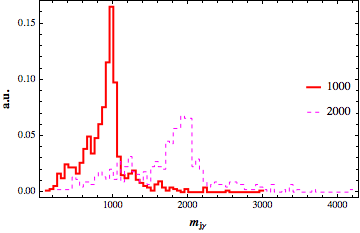
\includegraphics[width=7.2cm]{\main/section7OtherSignatures/img/pair1.png}&	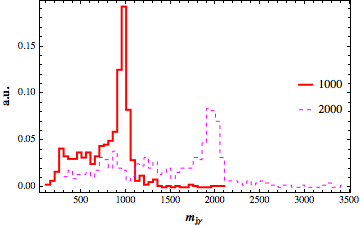
\includegraphics[width=7.2cm]{\main/section7OtherSignatures/img/pair2.png}
   			
   		\end{tabular}
   	\end{center}
   	\caption{Invariant mass $m_{j\gamma}$ for the two bench mark points. Left plot corresponds to the mass reconstruction with the 
	leading photon while the right is due to the sub-leading photon. Red line is for the 1 TeV mass case, while the dashed violet line is 
	for the 2 TeV mass for the colour octet scalar.}
   	\protect\label{fig:pair}
   \end{figure}
The acceptance efficiency for the 1 TeV point is $7\%$, while that for 2 TeV is $\sim 4\%$. For simulating the  background, 
QCD $pp\to j\gamma$, in the signal phase space, events are simulated requiring the scalar sum of the $p_T$ of the outgoing partons to be at least 500 GeV. This reduces the effective cross-section to be $660$ fb. Table \ref{tab:pair} gives summary of the acceptance efficiencies for signal and background. The mass reconstruction is not expected to change much at 27 TeV while the efficiencies may change. \\
 \begin{table}[h!]
 	\begin{center}
 		\begin{tabular}{|c|c|c|c|} 
 			\hline
 			
 			Cut flow           & QCD ($660~fb$)  & BP1&  BP2\\ \hline
 			\hline
 			
 			2 $\gamma$+2 jets         &0.005&0.07&0.02\\ \hline   
 		\end{tabular}
 		\caption{\label{tab:pair} Pair production efficiencies for signal and background. } 
 	\end{center}
 \end{table}

%\subsubsection{Single production}
%\paragraph*{Single production} 
The single production is characterized by the requirement of a single isolated photon and a jet. The benchmark considered in this case is $m_\Phi=1$ TeV. 
Figure \ref{fig:single} gives the distribution of different variables for this case: the top-left plot is the reconstruction of the photon-jet invariant mass. It is clear 
that this is a useful discriminator to distinguish signal from background. Thus it is enough to simulate the corresponding QCD events in the phase space 
of the signal where the effective cross-section of the former is reduced substantially. Other variables involving the photon and jet include: 1) The 
pseudo-rapidity difference $\Delta \eta_{j\gamma}=\eta_\gamma-\eta_j$ (top-right), 2) The difference in the azimuthal angle 
$\Delta \phi_{j\gamma}=\phi_\gamma-\phi_j$ (bottom-left), and 3) the angular distance $\Delta R_{j\gamma} =\sqrt{\Delta\eta_{j\gamma}^2+\Delta \phi_{j\gamma}} $.
Table \ref{tab:single} summarizes the efficiencies.
	\begin{figure}[htb!]
		\begin{center}
			\begin{tabular}{cc}
				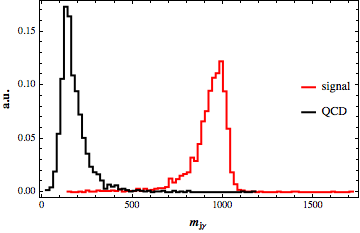
\includegraphics[width=7.2cm]{\main/section7OtherSignatures/img/single1.png}&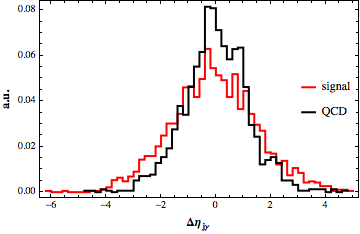
\includegraphics[width=7.2cm]{\main/section7OtherSignatures/img/single2.png}\\
				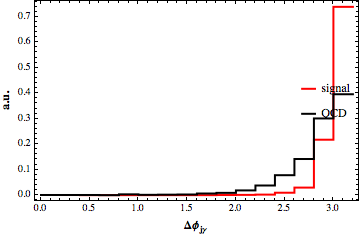
\includegraphics[width=7.2cm]{\main/section7OtherSignatures/img/single3.png}&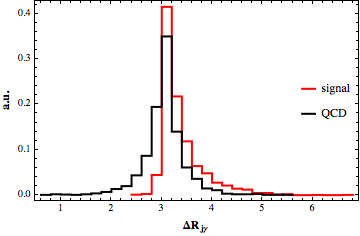
\includegraphics[width=7.2cm]{\main/section7OtherSignatures/img/single4.png}
			\end{tabular}
		\end{center}
		\caption{ Different variables for single production. See the text for a detailed description.}
		\protect\label{fig:single}
	\end{figure}
    
     \begin{table}[h!]
 	\begin{center}
 		\begin{tabular}{|c|c|c|} 
 			\hline
 			Cut flow           & QCD ($660~fb$)  & BP1\\ \hline
 			\hline
 			1 $\gamma$+1 jets         &0.40&0.18\\ \hline  
 			$700<m_(\gamma j) <1200$ GeV&0.17&.16 \\
 			\hline 
 		\end{tabular}
 		\caption{\label{tab:single}  Efficiencies for signal and background. } 
 	\end{center}
 \end{table}
%\subsubsection{Conclusion}
%\paragraph*{Conclusion}
 We have performed a simplified preliminary study of the potential for the study of pair and single production of a colour octet scalar decaying to gluon 
 and photon for two sample mass values of 1 and 2 TeV at the LHC. The naive comparison of the expected signal with respect to QCD background 
 shows that a discrimination of the signal over the background seems possible but requires a more detailed analysis.	
 
 %\bibliography{biblio}